\documentclass[12pt, a4paper, oneside, openright, titlepage]{book}
\usepackage[utf8]{inputenc}
\raggedbottom
\usepackage{import}


%%%%%%%%%%%%%%%%% Book Formatting Comments:

%%%%%%%%%%%%%%%%%%%%%%%%%%%%%%%%%%%%% for Part

%%%%%%%%%%%%%%%%%%%%%% for chapter

%%%%%%%%%%%%%%%%%%%% for section




%%%%%% PACKAGES %%%%%%%
\usepackage{hyperref}
\hypersetup{
    colorlinks,
    citecolor=black,
    filecolor=black,
    linkcolor=black,
    urlcolor=black
}
\usepackage{amsmath} % Math display options
\usepackage{amssymb} % Math symbols
%\usepackage{amsfonts} % Math fonts
%\usepackage{amsthm}
\usepackage{mathtools} % General math tools
\usepackage{array} % Allows you to write arrays
\usepackage{empheq} % For boxing equations
% \usepackage{mathabx}
% \usepackage{mathrsfs}
\usepackage{nameref}
\usepackage{wrapfig}

\usepackage{soul}
\usepackage[normalem]{ulem}

\usepackage{txfonts}
\usepackage{cancel}
\usepackage[toc, page]{appendix}
\usepackage{titletoc,tocloft}
\setlength{\cftchapindent}{1em}
\setlength{\cftsecindent}{2em}
\setlength{\cftsubsecindent}{3em}
%\setlength{\cftsubsubsecindent}{4em}
\usepackage{titlesec}

%\titleformat{\section}
%  {\normalfont\fontsize{25}{15}\bfseries}{\thesection}%{1em}{}
%\titleformat{\section}
%  {\normalfont\fontsize{20}{15}\bfseries}%{\thesubsection}{1em}{}
%\setcounter{secnumdepth}{1}  
  
  

%\newcommand\numberthis{\refstepcounter{equation}\tag{\theequation}} % For equation labelling
\usepackage[framemethod=tikz]{mdframed}

\usepackage{tikz} % For drawing commutative diagrams
\usetikzlibrary{cd}
\usetikzlibrary{calc}
\tikzset{every picture/.style={line width=0.75pt}} %set default line width to 0.75p

\usepackage{datetime}
\usepackage[margin=1.5in]{geometry}
\setlength{\parskip}{1em}
\usepackage{makeidx}         % allows index generation
\usepackage{graphicx}       % standard LaTeX graphics tool
\usepackage{multicol}        % used for the two-column index
\usepackage[bottom]{footmisc}% places footnotes at page bottom

\usepackage{newtxtext}       % 
\usepackage{newtxmath}       % selects Times Roman as basic font
\usepackage{float}
\usepackage{fancyhdr}
\setlength{\headheight}{15pt} 
\pagestyle{fancy}
\lhead[\leftmark]{}
\rhead[]{\leftmark}

%\usepackage{enumitem}

\usepackage{url}
\allowdisplaybreaks

%%%%%% ENVIRONMENTS %%%
\definecolor{purp}{rgb}{0.29, 0, 0.51}
\definecolor{bloo}{rgb}{0, 0.13, 0.80}



%%\newtheoremstyle{note}% hnamei
%{3pt}% hSpace above
%{3pt}% hSpace belowi
%{}% hBody fonti
%{}% hIndent amounti
%{\itshape}% hTheorem head fonti
%{:}% hPunctuation after theorem headi
%{.5em}% hSpace after theorem headi
%{}% hTheorem head spec (can be left empty, meaning ‘normal’)i





% %%%%%%%%%%%%% THEOREM DEFINITIONS

\spnewtheorem{axiom}{Axiom}[chapter]{\bfseries}{\itshape}


\spnewtheorem{construction}{Construction}[chapter]{\bfseries}{\itshape}

\spnewtheorem{props}{Properties}[chapter]{\bfseries}{\itshape}


\renewcommand{\qedsymbol}{$\blacksquare$}


\numberwithin{equation}{section}

\newenvironment{qest}{
    \begin{center}
        \em
    }
    {
    \end{center}
    }

%%%%%% MACROS %%%%%%%%%
%% New Commands
\newcommand{\ip}[1]{\langle#1\rangle} %%% Inner product
\newcommand{\abs}[1]{\lvert#1\rvert} %%% Modulus
\newcommand\diag{\operatorname{diag}} %%% diag matrix
\newcommand\tr{\mbox{tr}\.} %%% trace
\newcommand\C{\mathbb C} %%% Complex numbers
\newcommand\R{\mathbb R} %%% Real numbers
\newcommand\Z{\mathbb Z} %%% Integers
\newcommand\Q{\mathbb Q} %%% Rationals
\newcommand\N{\mathbb N} %%% Naturals
\newcommand\F{\mathbb F} %%% An arbitrary field
\newcommand\ste{\operatorname{St}} %%% Steinberg Representation
\newcommand\GL{\mathbf{GL}} %%% General Linear group
\newcommand\SL{\mathbf{SL}} %%% Special linear group
\newcommand\gl{\mathfrak{gl}} %%% General linear algebra
\newcommand\G{\mathbf{G}} %%% connected reductive group
\newcommand\g{\mathfrak{g}} %%% Lie algebra of G
\newcommand\Hbf{\mathbf{H}} %%% Theta fixed points of G
\newcommand\X{\mathbf{X}} %%% Symmetric space X
\newcommand{\catname}[1]{\normalfont\textbf{#1}}
\newcommand{\Set}{\catname{Set}} %%% Category set
\newcommand{\Grp}{\catname{Grp}} %%% Category group
\newcommand{\Rmod}{\catname{R-Mod}} %%% Category r-modules
\newcommand{\Mon}{\catname{Mon}} %%% Category monoid
\newcommand{\Ring}{\catname{Ring}} %%% Category ring
\newcommand{\Topp}{\catname{Top}} %%% Category Topological spaces
\newcommand{\Vect}{\catname{Vect}_{k}} %%% category vector spaces'
\newcommand\Hom{\mathbf{Hom}} %%% Arrows

\newcommand{\map}[2]{\begin{array}{c} #1 \\ #2 \end{array}}

\newcommand{\Emph}[1]{\textbf{\ul{\emph{#1}}}}




%% Math operators
\DeclareMathOperator{\ran}{Im} %%% image
\DeclareMathOperator{\aut}{Aut} %%% Automorphisms
\DeclareMathOperator{\spn}{span} %%% span
\DeclareMathOperator{\ann}{Ann} %%% annihilator
\DeclareMathOperator{\rank}{rank} %%% Rank
\DeclareMathOperator{\ch}{char} %%% characteristic
\DeclareMathOperator{\ev}{\bf{ev}} %%% evaluation
\DeclareMathOperator{\sgn}{sign} %%% sign
\DeclareMathOperator{\id}{Id} %%% identity
\DeclareMathOperator{\supp}{Supp} %%% support
\DeclareMathOperator{\inn}{Inn} %%% Inner aut
\DeclareMathOperator{\en}{End} %%% Endomorphisms
\DeclareMathOperator{\sym}{Sym} %%% Group of symmetries


%% Diagram Environments
\iffalse
\begin{center}
    \begin{tikzpicture}[baseline= (a).base]
        \node[scale=1] (a) at (0,0){
          \begin{tikzcd}
           
          \end{tikzcd}
        };
    \end{tikzpicture}
\end{center}
\fi




\newdateformat{monthdayyeardate}{%
    \monthname[\THEMONTH]~\THEDAY, \THEYEAR}
%%%%%%%%%%%%%%%%%%%%%%%

%%% Specific Macros %%%


%%%%%% BEGIN %%%%%%%%%%


\begin{document}

%%%%%% TITLE PAGE %%%%%

\begin{titlepage}
    \centering
    \scshape
    \vspace*{\baselineskip}
    \rule{\textwidth}{1.6pt}\vspace*{-\baselineskip}\vspace*{2pt}
    \rule{\textwidth}{0.4pt}
    
    \vspace{0.75\baselineskip}
    
    {\LARGE Theoretical Computer Science: A Complete Guide}
    
    \vspace{0.75\baselineskip}
    
    \rule{\textwidth}{0.4pt}\vspace*{-\baselineskip}\vspace{3.2pt}
    \rule{\textwidth}{1.6pt}
    
    \vspace{2\baselineskip}
    Computer Science \\
    \vspace*{3\baselineskip}
    \monthdayyeardate\today \\
    \vspace*{5.0\baselineskip}
    
    {\scshape\Large Elijah Thompson, \\ Physics and Math Honors\\}
    
    \vspace{1.0\baselineskip}
    \textit{Solo Pursuit of Learning}
    \vfill
    \enlargethispage{1in}
    \begin{figure}[b!]
    \makebox[\textwidth]{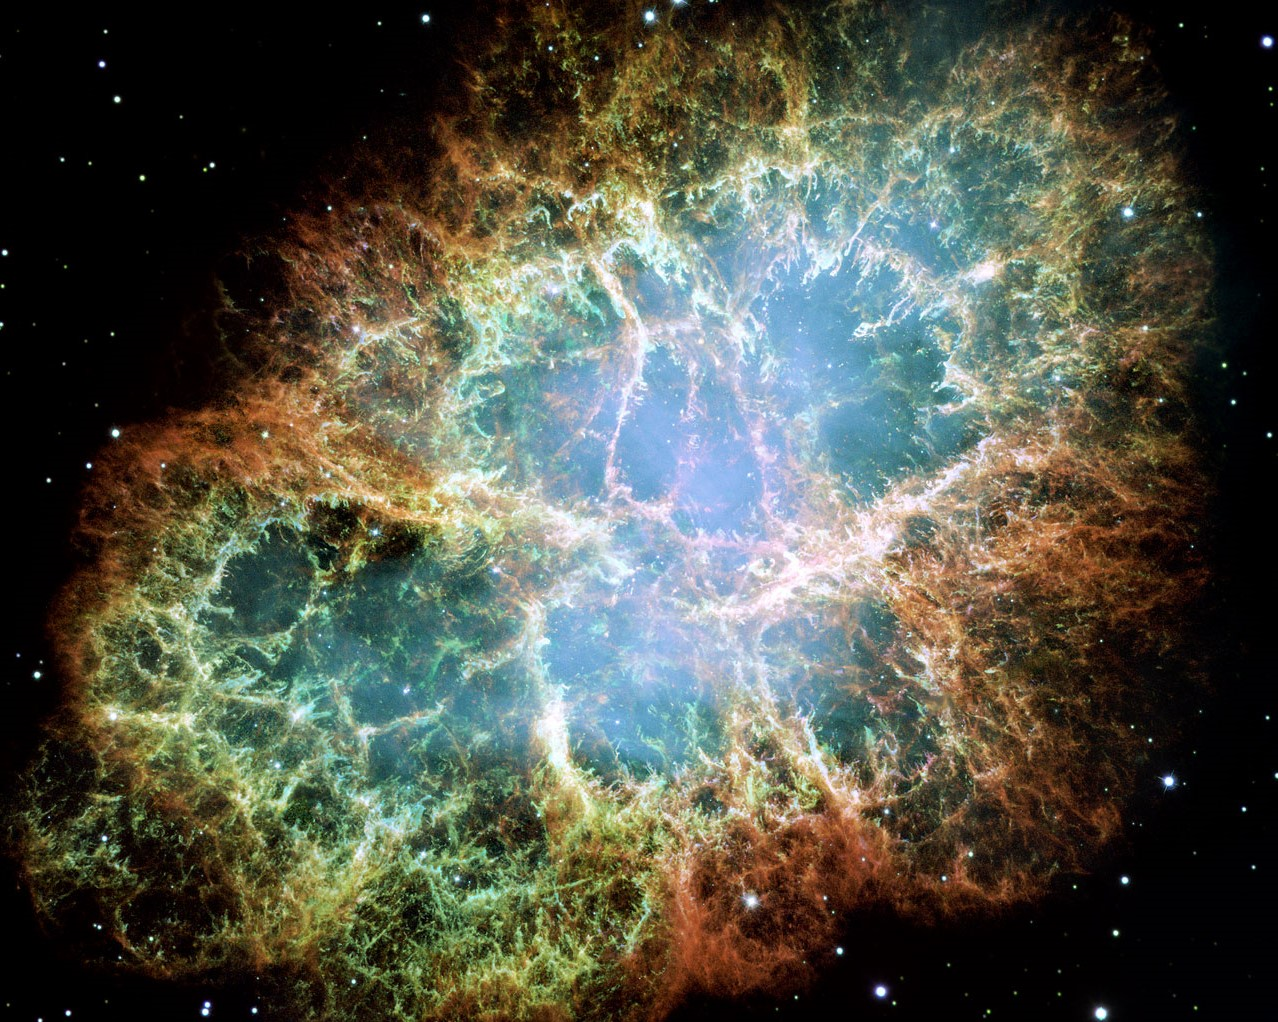
\includegraphics[width=\paperwidth, height =10cm]{../Crab.jpg}}
    \end{figure}
\end{titlepage}

%%%%%%%%%%%%%%%%%%%%%%%
\tableofcontents

%%%%%%%%%%%%%%%%%%%%%%%%%%%%%%%%%%%%% Part 1.
\part{Comp Phys 381}

%%%%%%%%%%%%%%%%%%%%%%% - Chapter 1.1
\chapter{Root Finding Methods}



\section{Bisection Method}

\begin{proc}
	To find the roots of a function $f$ we first choose a pair of initial values $x_B$ and $x_U$ such that $f(x_B) < 0$ and $f(x_U) > 0$. Then we perform the following iterative procedure:
	\begin{enumerate}
		\item Define $x_C = \frac{x_B+x_U}{2}$, and evaluate $f(x_C)$.
		\item If $f(x_C) > 0$ set $x_U = x_C$
		\item If $f(x_C) < 0$ set $x_B = x_C$
		\item Repeat until $|f(x_C)|$ is less than some chosen tolerance, $\epsilon$.
	\end{enumerate}
\end{proc}


\section{Newton-Raphson Method}

\begin{proc}
        Consider a real valued function $f$. Note that the Taylor expansion of $f$ centered at a point $x_0$ and evaluated at $x_0 + \epsilon$ is \begin{equation}
                f(x_0+\epsilon) = f(x_0) + f'(x_0)\epsilon + \frac{1}{2}f''(x_0)\epsilon^2 + ... = \sum_{n=0}^{\infty}\frac{f^{(n)}(x_0)\epsilon^n}{n!}
        \end{equation}
        With the NR Method $x_0$ is the current estimate for the root of our function. We now truncate the series to terms linear in $\epsilon$: \begin{equation}
                f(x_0+\epsilon) = f(x_0) + f'(x_0)\epsilon + O(\epsilon^2)
        \end{equation}
        where $O(\epsilon^2)$ indicates that the terms of order $\epsilon^2$ and higher are omitted. We set $f(x_0+\epsilon) = 0$. This gives \begin{equation}
                f(x_0) + f'(x_0)\epsilon = 0
        \end{equation}
        from which we obtain \begin{equation}
                \epsilon_0 = -\frac{f(x_0)}{f'(x_0)}
        \end{equation}
        setting $\epsilon = \epsilon_0$. We then let $x_1 = x_0 + \epsilon_0$ and calculate a new $\epsilon_1$. We extend this process and define it recursively as \begin{equation}
                x_{n+1} = x_n - \frac{f(x_n)}{f'(x_n)}
        \end{equation}
        for an indexing ineger $n \geq 0$.
\end{proc}




%%%%%%%%%%%%%%%%%%%%%%% - Chapter 1.2
\chapter{Non-Linear ODEs}

\begin{rmk}
        In this chapter considered the differential equation described by \begin{equation}
                \frac{dx}{dt} = y, \;\;\frac{dy}{dt} = f(x,y,t)
        \end{equation}
\end{rmk}


\section{Euler Method}

\begin{proc}
        We first choose initial conditions $x(0) = x_0$ and $y(0) = y_0$. Consider the Taylor series expansion of a function $g$ about $a+h$ centered at $a$:\begin{equation}
                f(a+h) = f(a) + hf'(a) + \frac{h^2}{2!}f''(a) + O(h^3)
        \end{equation}
        We apply this to $x(t)$ and $y(t)$ to obtain \begin{align}
                x(t + \Delta t) &= x(t) + \Delta t \frac{dx(t)}{dt} + O(\Delta t^2)\\
                y(t + \Delta t) &= y(t) + \Delta t \frac{dy(t)}{dt} + O(\Delta t^2)
        \end{align}
        where we omit terms of order $\Delta t^2$. We shall vary $t$ steps discretely and label $\Delta t = t_{n-1} - t_n$, so our equations of motion become \begin{align}
                x_{n+1} &= x_n + y_n\Delta t \\
                y_{n+1} &= y_n + f(x_n,y_n,t_n)\Delta t
        \end{align}
        using Euler's Method for approximating integrals. In particular, for Euler's method we take \begin{equation}
                g(b) - g(a) = \int_a^b\frac{dg}{dt}dt \approx \sum_{i=1}^n\frac{dg(t_i)}{dt}\Delta t, t_1 = a, t_n = b - \Delta t
        \end{equation}
\end{proc}


\section{Trapezoid Rule}


\begin{proc}
        For the trapezoid rule we approximate an integral as follows \begin{equation}
                (b-a)\left[\frac{\frac{dg(a)}{dt} + \frac{dg(b)}{dt}}{2}\right] \approx \int_a^b\frac{dg}{dt}dt = g(b) - g(a)
        \end{equation}
        Then, applying this to our DE we obtain the iterative equation \begin{equation}
                x_{n+1} \approx x_n + \frac{\Delta t}{2}\left(y_n + y_{n+1}\right)
        \end{equation}
        where $\Delta t = t_{n+1} - t_n$. We then approximate $y_{n+1}$ using Euler's Method \begin{equation}
                y_{n+1} \approx y_n + \Delta t f(x_n,y_n, t_n)
        \end{equation}
        Substituting this back into our previous approximation for $x_{n+1}$ we have \begin{equation}
                x_{n+1} \approx x_n + \frac{\Delta t}{2}\left[y_n + (y_n + \Delta tf(x_n,y_n,t_n)\right]
        \end{equation}
        We apply this again to $y_{n+1}$ to obtain the approximation \begin{equation}
                y_{n+1} \approx y_n + \frac{\Delta t}{2}\left[f(x_n,y_n,t_n) + \delta tf(x_{n+1},y_n + \Delta tf(x_n,y_n,t_n), t_{n+1})\right]
        \end{equation}
        This pair of iterative equations constitute the application of the trapezoid rule to solving our DE.
\end{proc}


\section{Runge-Kutta}


\begin{proc}[Second Order]
        We first carry out a Taylor expansion of $\frac{dx(t)}{dt}$ about the midpoints of our interval, $\Delta t/2$: \begin{equation}
                \frac{dx(t)}{dt} = \frac{dx(\Delta t/2)}{dt} + \frac{d^2x(\Delta t/2)}{dt^2}(t - \Delta t/2) + O\left(\frac{\Delta t}{2}^2\right)
        \end{equation}
        We use this expansion to approximate the following integral:\begin{equation}
                \int_{0}^{\Delta t}\frac{x(t)}{dt}dt \approx \frac{dx(\Delta t/2)}{dt}\Delta t + \frac{d^2x(\Delta t/2)}{dt^2}\int_{0}^{\Delta t}(t-\Delta t/2)dt = \frac{dx(\Delta t/2)}{dt}\Delta t
        \end{equation}
        Then, the rule to update $x$ in an algorithmic notation is given by \begin{equation}
                x_{n+1} \approx x_n + y_{n+1/2}\Delta t + O\left(\frac{\Delta t}{2}^2\right)
        \end{equation}
        and applying the Taylor expansion to $y_{n+1/2}$ we have \begin{equation}
                y_{n+1/2} \approx = y_n + f(x_n,y_n,t_n)\frac{\Delta t}{2} + O\left(\frac{\Delta t}{2}^2\right)
        \end{equation}
        Substituing into our $x_{n+1}$ rule we have \begin{equation}
                x_{n+1} \approx x_n + \left( y_n + f(x_n,y_n,t_n)\frac{\Delta t}{2}\right)\Delta t
        \end{equation}
        The rule for updating $y_n$ is given by \begin{align}
                y_{n+1} &= y_n + f(x_{n+1/2},y_{n+1/2},t_{n+1/2})\Delta t \\
                y_{n+1/2} &= y_n + f(x_n,y_n,t_n)\frac{\Delta t}{2} \\
                x_{n+1/2} &= x_n + y_n\frac{\Delta t}{2} 
        \end{align}
\end{proc}


\begin{proc}[Fourth Order]
        In implementing we take a series of approximations for $x_n$ and $y_n$ then take a weighted average of the result. In particular, we take the approximations \begin{align}
                k_{1x,n} &= \Delta t y_n \\
                k_{1y,n} &= \Delta t f(x_n,y_n,t_n) \\
                k_{2x,n} &= \Delta t \left(y_n+ \frac{k_{1y,n}}{2}\right) \\
                k_{2y,n} &= \Delta tf\left(x_n + \frac{k_{1x,n}}{2}, y_n + \frac{k_{1y,n}}{2}, t_n + \Delta t/2\right) \\
                k_{3x,n} &= \Delta t\left(y_n+ \frac{k_{2y,n}}{2}\right) \\
                k_{3y,n} &= \Delta t f\left(x_n + \frac{k_{2x,n}}{2}, y_n + \frac{k_{2y,n}}{2}, t_n + \Delta t/2\right) \\
                k_{4x,n} &= \Delta t \left(y_n + k_{3y,n}\right)\\
                k_{4y,n} &= \Delta tf\left(x_n + k_{3x,n}, y_n + k_{3y,n}, t_n + \Delta t\right) \\
                x_{n+1} &= x_n + \frac{k_{1x,n} + 2k_{2x,n} + 2k_{3x,n} + k_{4x,n}}{6} \\
                y_{n+1} &= y_n + \frac{k_{1y,n} + 2k_{2y,n} + 2k_{3y,n} + k_{4y,n}}{6} 
        \end{align}
\end{proc}






%%%%%%%%%%%%%%%%%%%%%%% - Chapter 1.3
\chapter{Numerical Fourier Analysis}


\section{Fourier Series}


\begin{defn}[Fourier Series]
        Any periodic function $f(t)$ with period $T = 2\pi/\omega$ can be represented as a \Emph{Fourier Series}\begin{equation}
                f(t) = a_0 + \sum_{n=1}^{\infty}\left[a_n\cos(n\omega t) + b_n\sin(n\omega t)\right]
        \end{equation}
        The frequency $\omega$ is known as the \Emph{fundamental frequency} and $\omega_n = n\omega$ for $n >1$ are the \Emph{harmonics}. The result of Fourier-analysing a signal is a set of values for these coefficients for all $n$.
\end{defn}

\begin{proc}
        The Fourier coefficients for a periodic function $f$ are evaluated using the orthogonality properties of sines and cosines:\begin{align}
                \frac{2}{T}\int_0^T\sin(n\omega t)\sin(k\omega t)dt &= \delta_{nk} \\
                \frac{2}{T}\int_0^T\cos(n\omega t)\sin(k\omega t)dt &= 0 \\
                \frac{2}{T}\int_0^T\cos(n\omega t)\cos(k\omega t)dt &= \delta_{nk}
        \end{align}
        Applying these orthogonality properties we obtain the following equations for the coefficients:\begin{align}
                a_0 &= \frac{1}{T}\int_0^Tf(t)dt \\
                a_k &= \frac{2}{T}\int_0^Tf(t)\cos(k\omega t)dt, k \in \{1,2,3,...\} \\
                b_k &= \frac{2}{T}\int_0^Tf(t)\sin(k\omega t)dt, k\in \{1,2,3,...\}
        \end{align}
\end{proc}


\section{Simpson's Rule}

\begin{proc}
        Simpson's rule is a method of numerical integration. In particular, to approximate the integral $\int_a^bf(x)dx$ we split the interval $[a,b]$ into $n$ steps of length $h = (b-a)/n$, where $n \in 2\Z$. The approximation is taken as \begin{equation}
                \int_a^bf(t)dt \approx \frac{h}{3}\left[ f(x_0) + 2\sum_{j=1}^{n/2-1}f(x_{2j}) + 4\sum_{j=1}^{n/2}f(x_{2j-1}) + f(x_n)\right]
        \end{equation}
        where $x_j = a + jh$ for $j \in \{0,1,2,...,n-1, n\}$. In particular $x_0 = a$ and $x_n = b$.
\end{proc}


\section{Fourier Integral}

\begin{rmk}
        For a non-periodic function $f(t)$ we require a \Emph{Fourier integral} over a continuous range of frequencies. The Fourier integral may be viewed as a limit of a Fourier series in the limit $T\rightarrow \infty$.
\end{rmk}


\begin{proc}
        For a non periodic function $f(t)$ its Fourier integral is given by \begin{equation}
                f(t) = \int_0^{\infty}\left[a(\omega)\cos(\omega t) + b(\omega)\sin(\omega t)\right]d\omega
        \end{equation}
        and the coefficient equations become functions of $\omega$:\begin{align}
                a(\omega) &= \frac{1}{\pi}\int_{-\infty}^{\infty}f(t)\cos(\omega t)dt \\
                b(\omega) &= \frac{1}{\pi}\int_{-\infty}^{\infty}f(t)\sin(\omega t)dt
        \end{align}
        Using Euler's identity $e^{i\omega t} = \cos(\omega t) + i\sin(\omega t)$ we can rewrite this as \begin{align}
                f(t) &= \frac{1}{\sqrt{2\pi}}\int_{-\infty}^{\infty}F(\omega)e^{i\omega t}d\omega \\
                F(\omega) &= \frac{1}{\sqrt{2\pi}}\int_{-\infty}^{\infty}f(t)e^{-i\omega t}dt
        \end{align}
        where $F(\omega)$ is the \Emph{Fourier Transform} of $f(t)$. If the signal has dimensions of energy, then its Fourier Transform has units of Power, and its magnitude $|F(\omega)|$ is a measure of the total power in the signal at frequency $\omega$: \begin{equation}
                |F(\omega)| = \sqrt{\R e\{F(\omega)\}^2+\mathbb{I}m\{F(\omega)\}^2} = \sqrt{\pi}{2}\sqrt{a^2(\omega) + b^2(\omega)}
        \end{equation}
\end{proc}


\section{Discrete Fourier Transform}

\begin{defn}
        In practice we approximate the Fourier integral and its other corresponding forms using finite summations, known as the \Emph{Discrete Fourier Transform}. Let $f(t)$ be a non-periodic function that we have $N$ samples of at intervals $h$ going from $t = 0$ to $t = (N-1)h$. We define a discrete timeline by $t_m = mh$ for $m \in \{0,1,2,...,N-1\}$. The time $\tau = Nh$ will become the period of our approximated function under reconstruction, and we need $\tau$ to be the longest time over which we are interested in the behaviour of $f(t)$. We also assume \begin{equation}
                f(t) = f(t+\tau) \iff f(t_m) = f(t_{m+N}) \iff f_m = f_{m+N}
        \end{equation}
        The lowest frequency in the DFT will be $\nu_1 = 1/\tau = 1/(Nh)$, and this will be the fundamental frequency of our reconstructed function. The frequency spectrum is given by \begin{equation}
                \Lambda := \left\{\nu_n = \frac{n}{Nh} = n\nu_1\vert n \in \N\right\}
        \end{equation}
        We then discretize the integrals for the function and its Fourier transform as \begin{align}
                f_m &= frac{1}{N}\sum_{n=0}^{N-1}F_ne^{i2\pi\nu_nt_m} = \frac{1}{N}\sum_{n=0}^{N-1}F_ne^{i2\pi mn/N} \\
                F_n &= \sum_{m=0}^{N-1}f_me^{-i2\pi\nu_nt_m} = \sum_{m=0}^{N-1}f_me^{-2\pi mn/N}
        \end{align}
        Note that it can be shown that $F_{N/2-n} = \overline{F}_{N/2+n}$ for $n \in \{0,1,...,N/2\}$. The highest frequency component is thus $F_{N/2-1}$, corresponding to a frequency of \begin{equation}
                \nu_{max} = (N/2-1)/Nh = 1/(2h) - 1/(Nh) \approx 1/(2h), \text{ if $N$ large}
        \end{equation}
        This is also known as the \Emph{nyquist frequency} $\nu_{Nyquist}$.


        If the function has a component with frequency $\nu > \nu_{Nyquist}$ there are less than two sample points per period. This implies that there will be one or more frequencies less than $\nu_{Nyquist}$ for which the amplitude equals the true amplitude at the sample points, but these lower frequencies are not in the signal although they will appear in the frequency spectrum - this is phenomenon known as \Emph{aliasing}. The power spectrum of the DFT is often plotted as all values \begin{equation}
                P_n = |F_n|^2 = \R e\{F_n\}^2+\mathbb{I}m\{F_n\}^2
        \end{equation}
\end{defn}


\begin{proc}
        In application we use the following summations for the components of $F_n$ \begin{align}
                \R e\{F_n\} &= \sum_{m=0}^{N-1}f_m\cos\left(\frac{2\pi mn}{N}\right) \\
                \mathbb{I}m\{F_n\} &= \sum_{m=0}^{N-1}f_m\sin\left(\frac{2\pi mn}{N}\right)
        \end{align}
        We then reconstruct the original signal as \begin{equation}
                f_m = \frac{1}{N}\sum_{n=0}^{N-1}\left\{\R e\{F_n\}\cos\left(\frac{2\pi mn}{N}\right) + \mathbb{I}m\{F_n\}\sin\left(\frac{2\pi mn}{N}\right)\right\}
        \end{equation}
\end{proc}




%%%%%%%%%%%%%%%%%%%%%%% - Chapter 1.4
\chapter{Curve-fitting and Optimization}


\section{Least Squares}

\begin{proc}
        Assume we have some sequence of measurements at times $t_i$ \begin{equation}
                y_i = y(t_i)
        \end{equation}
        and for some presumed model of the relationship \begin{equation}
                ~y = f(t;p)
        \end{equation}
        expressed in terms of the independent variable $t$ and the model parameters $p$. We define the distance between a data point and our model by \begin{equation}
                \delta_i = y_i - ~y_i
        \end{equation}
        A general measure of the distance is \begin{equation}
                \sum_i|\delta_i|^d
        \end{equation}
        For $d = 2$ we obtain the \Emph{chi-squared} measure \begin{equation}
                \chi^2 = \sum_i|y_i - ~y_i(p_1,...,p_K)|^2
        \end{equation}
        The best fit is assumed to minimize $\chi^2$ with respect to the model parameters \begin{equation}
                \frac{\partial \chi^2}{\partial p_l} = \sum_i2|y_i - ~y_i(p_1,...,p_K)|\frac{\partial ~y_i}{\partial p_l}
        \end{equation}
        We also usually use the \Emph{reduce chi-squared} value \begin{equation}
                \chi^2_N = \frac{\chi^2}{N}
        \end{equation}
        In general we want $\chi^2$ to scale with the uncertainty in our measurements, so we wish to minimize \begin{equation}
                \sum\left(\frac{expected-observed}{uncertainty}\right)^2
        \end{equation}
\end{proc}

\begin{rmk}
        This minimization can be done numerically using \Emph{scipy.optimize} package's \Emph{minimize} method. This package also has a \Emph{curve\_fit} method for non-linear data sets.
\end{rmk}

\section{Finite Differences}


\begin{proc}
        Consider a real-valued function $f(x)$ and its Taylor series about some point $x=a$:\begin{equation}
                f(x) = \sum_{n=0}^{\infty}\frac{f^{(n)}(a)}{n!}(x-a)^n
        \end{equation}
        Consider a set of points, $x_i$, such that $x_{i+1} = x_i + \Delta$. Then we have that \begin{equation}
                f(x_{i+n}) = f(x_i) + f'(x_i)n\Delta + \frac{f''(x_i)}{2!}(n\Delta)^2+\frac{f'''(x_i)}{3!}(n\Delta)^3+O(\Delta^4)
        \end{equation}
        Define $f(x_{i+n}) =: f_{i+n}$. Then for neighboring points we have \begin{align}
                f_{i+1} = f_i+f'_i\Delta +\frac{f''_i}{2!}\Delta^2 + \frac{f_i'''}{3!}\Delta^3 + O(\Delta^4) \\
                f_i = f_i \\
                f_{i-1} = f_i-f'_i\Delta +\frac{f''_i}{2!}\Delta^2 - \frac{f_i'''}{3!}\Delta^3 + O(\Delta^4)
        \end{align}
        Subtracting the expression for two neighboring points we have \begin{equation}
                f_{i+1} - f_i = f'_i\Delta +\frac{f''_i}{2!}\Delta^2 + \frac{f_i'''}{3!}\Delta^3 + O(\Delta^4)
        \end{equation}
        Dividing by $\Delta$ we obtain the following \Emph{forward difference} estimate of the first derivative \begin{equation}
                \frac{f_{i+1} - f_i}{\Delta} = f'_i+\frac{f''_i}{2!}\Delta + \frac{f_i'''}{3!}\Delta^2 + O(\Delta^3) \approx f'_i + O(\Delta)
        \end{equation}
        Similarly we obtain the \Emph{backward difference} estimate \begin{equation}
                f'_i \approx \frac{f_i - f_{i-1}}{\Delta} + O(\Delta)
        \end{equation}
        We can also cancel all even terms in the expansion by \begin{equation}
                f_{i+1} - f_{i-1} = 2f'_i\Delta +2\frac{f'''_i}{3!}\Delta^3+O(\Delta^5)
        \end{equation}
        which gives us the \Emph{centered difference} estimate \begin{equation}
                f'_i \approx \frac{f_{i+1} - f_{i-1}}{2\Delta} + O(\Delta^2)
        \end{equation}
        By adding terms we can cancel all odd terms and obtain \begin{equation}
                f_{i+1} + f_{i-1} = 2f_i + 2\frac{f''_i}{2!}\Delta^2 + O(\Delta^4)
        \end{equation}
        We then obtain an expression for the \Emph{second difference} estimate \begin{equation}
                f''_i = \frac{f_{i+1} - 2f_i + f_{i-1}}{\Delta^2} + O(\Delta^2)
        \end{equation}
\end{proc}












%%%%%%%%%%%%%%%%%%%%%%%%%%%%%%%%%%%%% Part 3.
\part{Computability}

%%%%%%%%%%%%%%%%%%%%%%% - Chapter 3.1
\chapter{Automata and Languages}


\section{Finite Automata}

In general, finite automata are good models for computers with an extremely limited amount of memory. Finite automata and their probabilistic counterpart \Emph{Markov chains} are useful tools when we are attempting to recognize patterns in data. 

A \Emph{state diagram} of a finite automaton $M_1$ is a diagram with several states and labeled arrows depicting transitions between states.
\begin{center}
    \begin{tikzpicture}[x=0.75pt,y=0.75pt,yscale=-1,xscale=1]
%uncomment if require: \path (0,288); %set diagram left start at 0, and has height of 288

%Flowchart: Connector [id:dp6087132957460275] 
\draw   (113.78,137.33) .. controls (113.78,123.16) and (125.05,111.67) .. (138.94,111.67) .. controls (152.84,111.67) and (164.11,123.16) .. (164.11,137.33) .. controls (164.11,151.51) and (152.84,163) .. (138.94,163) .. controls (125.05,163) and (113.78,151.51) .. (113.78,137.33) -- cycle ;
%Flowchart: Connector [id:dp7390461236495558] 
\draw   (229.78,137.33) .. controls (229.78,123.16) and (241.05,111.67) .. (254.94,111.67) .. controls (268.84,111.67) and (280.11,123.16) .. (280.11,137.33) .. controls (280.11,151.51) and (268.84,163) .. (254.94,163) .. controls (241.05,163) and (229.78,151.51) .. (229.78,137.33) -- cycle ;
%Flowchart: Connector [id:dp8773846520603694] 
\draw   (333.11,135.33) .. controls (333.11,121.16) and (344.38,109.67) .. (358.28,109.67) .. controls (372.18,109.67) and (383.44,121.16) .. (383.44,135.33) .. controls (383.44,149.51) and (372.18,161) .. (358.28,161) .. controls (344.38,161) and (333.11,149.51) .. (333.11,135.33) -- cycle ;
%Flowchart: Connector [id:dp9560904959564065] 
\draw   (232.44,137.33) .. controls (232.44,125) and (242.52,115) .. (254.94,115) .. controls (267.37,115) and (277.44,125) .. (277.44,137.33) .. controls (277.44,149.67) and (267.37,159.67) .. (254.94,159.67) .. controls (242.52,159.67) and (232.44,149.67) .. (232.44,137.33) -- cycle ;
%Straight Lines [id:da8063038689848527] 
\draw    (50.78,135.67) -- (106.78,136.31) ;
\draw [shift={(108.78,136.33)}, rotate = 180.66] [color={rgb, 255:red, 0; green, 0; blue, 0 }  ][line width=0.75]    (10.93,-3.29) .. controls (6.95,-1.4) and (3.31,-0.3) .. (0,0) .. controls (3.31,0.3) and (6.95,1.4) .. (10.93,3.29)   ;
%Curve Lines [id:da7380519374583219] 
\draw    (121.44,118.33) .. controls (124.74,80.71) and (155.49,73.15) .. (156.75,119.58) ;
\draw [shift={(156.78,121)}, rotate = 269.2] [color={rgb, 255:red, 0; green, 0; blue, 0 }  ][line width=0.75]    (10.93,-3.29) .. controls (6.95,-1.4) and (3.31,-0.3) .. (0,0) .. controls (3.31,0.3) and (6.95,1.4) .. (10.93,3.29)   ;
%Curve Lines [id:da1257198526259986] 
\draw    (164.11,137.33) .. controls (183.61,112.31) and (211.98,118.65) .. (228.53,135.98) ;
\draw [shift={(229.78,137.33)}, rotate = 228.3] [color={rgb, 255:red, 0; green, 0; blue, 0 }  ][line width=0.75]    (10.93,-3.29) .. controls (6.95,-1.4) and (3.31,-0.3) .. (0,0) .. controls (3.31,0.3) and (6.95,1.4) .. (10.93,3.29)   ;
%Curve Lines [id:da4075876046436395] 
\draw    (280.11,137.33) .. controls (299.61,112.31) and (315.94,116.75) .. (331.89,133.98) ;
\draw [shift={(333.11,135.33)}, rotate = 228.3] [color={rgb, 255:red, 0; green, 0; blue, 0 }  ][line width=0.75]    (10.93,-3.29) .. controls (6.95,-1.4) and (3.31,-0.3) .. (0,0) .. controls (3.31,0.3) and (6.95,1.4) .. (10.93,3.29)   ;
%Curve Lines [id:da23711215049537637] 
\draw    (281.34,138.95) .. controls (294.88,156.12) and (317.92,162.93) .. (333.44,139) ;
\draw [shift={(280.11,137.33)}, rotate = 53.97] [color={rgb, 255:red, 0; green, 0; blue, 0 }  ][line width=0.75]    (10.93,-3.29) .. controls (6.95,-1.4) and (3.31,-0.3) .. (0,0) .. controls (3.31,0.3) and (6.95,1.4) .. (10.93,3.29)   ;
%Curve Lines [id:da22457745027273757] 
\draw    (237.44,118.33) .. controls (240.74,80.71) and (270.18,69.88) .. (271.42,116.24) ;
\draw [shift={(271.44,117.67)}, rotate = 269.2] [color={rgb, 255:red, 0; green, 0; blue, 0 }  ][line width=0.75]    (10.93,-3.29) .. controls (6.95,-1.4) and (3.31,-0.3) .. (0,0) .. controls (3.31,0.3) and (6.95,1.4) .. (10.93,3.29)   ;

% Text Node
\draw (133.11,130.4) node [anchor=north west][inner sep=0.75pt]    {$q_{1}$};
% Text Node
\draw (248.44,129.07) node [anchor=north west][inner sep=0.75pt]    {$q_{2}$};
% Text Node
\draw (352.44,125.73) node [anchor=north west][inner sep=0.75pt]    {$q_{3}$};
% Text Node
\draw (136.44,74.4) node [anchor=north west][inner sep=0.75pt]  [font=\scriptsize]  {$0$};
% Text Node
\draw (190.44,109.73) node [anchor=north west][inner sep=0.75pt]  [font=\scriptsize]  {$1$};
% Text Node
\draw (301.11,107.73) node [anchor=north west][inner sep=0.75pt]  [font=\scriptsize]  {$0$};
% Text Node
\draw (300.44,157.73) node [anchor=north west][inner sep=0.75pt]  [font=\scriptsize]  {$0,1$};
% Text Node
\draw (251.11,71.07) node [anchor=north west][inner sep=0.75pt]  [font=\scriptsize]  {$1$};


\end{tikzpicture}
\end{center}

The \Emph{start state} is indicated by an arrow pointing at it from nowhere. The \Emph{accept state} is the one with a double circle, and the arrows going from one state to another are called \Emph{transitions}.

A finite automaton consists of a set of states and rules for going between states depending on the input symbol; an input alphabet that indicates the allowed input symbols; a start state and a set of accept states; and a \Emph{transition function}, $\delta$, which takes in a state and an input symbol and outputs another state: $\delta(state_1,input)= state_2$. Formally, we have 

\begin{defn}
    A \Emph{finite automaton} is a 5-tuple $(Q,\sum,\delta,q_0,F)$, where \begin{enumerate}
        \item $Q$ is a finite set called the \Emph{states}
        \item $\sum$ is a finite set called the \Emph{alphabet}
        \item $\delta:Q\times \sum\rightarrow Q$ is the \Emph{transition function}
        \item $q_0 \in Q$ is the \Emph{start state}, and 
        \item $F \subseteq Q$ is the \Emph{set of accept states}
    \end{enumerate}
\end{defn}

If $A$ is the set of all strings that machine $M$ accepts, we say that $A$ is the \Emph{language of machine $M$} and write $L(M) = A$. We say that \Emph{$M$ recognizes $A$} or that \Emph{$M$ accepts $A$}.

A machine may accept several strings, but it always recognizes only one language. 

Let $M = (Q,\sum,\delta, q_0, F)$ be a finite automaton and let $w = w_1w_2...w_n$ be a string where each $w_i$ is a member of the alphabet $\sum$. Then $M$ \Emph{accepts} $w$ if a sequence of states $r_0,r_1,...,r_n$ in $Q$ exists satisfying three conditions: \begin{enumerate}
    \item $r_0 = q_0$
    \item $\delta(r_i,w_{i+1}) = r_{i+1}$, for $i = 0,...,n-1$
    \item $r_n \in F$.
\end{enumerate}

We say that \Emph{$M$ recognizes language $A$} if $A = \{w\vert M\;\text{ accepts }\; w\}$.

\begin{defn}
    A language is called a \Emph{regular language} if some finite automaton recognizes it.
\end{defn}

When designing an automaton it is best to put yourself in the place of the machine, seeing how you would perform the tasks you need the machine to. Once you have determined the necessary information to remember about the string as it is being read, you represent this information as a finite list of possibilities, and assign a state to each of the possibilites. 


In the theory of computation, the objects are languages and the tools include operations specifically designed for manipulating them. We define three operations on languages, called the \Emph{regular operations}, and use them to study properties of regular languages: \begin{defn}
    Let $A$ and $B$ be languages. We define the regular operations \Emph{union}, \Emph{concatenation}, and \Emph{star} as follows: \begin{itemize}
        \item \Emph{Union:} $A\cup B = \{x\vert x \in A\lor x \in B\}$
        \item \Emph{Concatenation:} $A\circ B = \{xy\vert x \in A\land y \in B\}$
        \item \Emph{Star:} $A^* = \{x_1x_2...x_k\vert k \geq 0\;\text{ and each }\;x_i \in A\}$.
    \end{itemize}
\end{defn}

\begin{thm}
    The class of regular languages is closed under the union operation. In other words, if $A_1$ and $A_2$ are regular languages, so is $A_1\cup A_2$.
\end{thm}
\begin{proof}[Sketch]
    We have regular languages $A_1$ and $A_2$ and want to show $A_1 \cup A_2$ is regular. Let $M_1 = (Q_1,\sum,\delta_1,q_1,F_1)$ be the finite automata that recognizes $A_1$, and let $M_2 = (Q_2,\sum,\delta_2,q_2,F_2)$ be the finite automata that recognizes $A_2$. Construct $M = (Q,\sum,\delta,q_0,F)$ as follows: \begin{enumerate}
        \item Let $Q = \{(r_1,r_2)\vert r_1 \in Q_1\land r_2 \in Q_2\} = Q_1\times Q_2$.
        \item $\sum$, the alphabet, is the same as in both automatas. Even if the automata had different alphabets $\sum_1$ and $\sum_2$, we would simply take $\sum = \sum_1\cup \sum_2$.
        \item $\delta$, the transition function, is defined for all $(r_1,r_2) \in Q$ and $a \in \sum$ by \begin{equation*}
                \delta((r_1,r_2),a) = (\delta_1(r_1,a),\delta_2(r_2,a))
            \end{equation*}
        \item $q_0$ is the pair $(q_1,q_2)$
        \item $F$ is the set of pairs in which either member is an accept state of $M_1$ or $M_2$. We can write it as \begin{equation*}
                F = \{(r_1,r_2)\vert r_1 \in F_1\lor r_2 \in F_2\}
        \end{equation*}
        This expression is the same as $F= (F_1\times Q_2)\cup(Q_1\times F_2)$.
    \end{enumerate}
    By construction it follows that $M$ is a finite automaton which recognizes the union of $A_1$ and $A_2$.
\end{proof}

\begin{thm}
    The class of regular languages is closed under the concatenation operation. In other words, if $A_1$ and $A_2$ are regular languages then so is $A_1 \circ A_2$.
\end{thm}

To prove this theorem we must learn some more techniques.


\section{Nondeterminism}


So far in our discussion, every step of a computation follows in a unique way from the preceding step. 

\begin{defn}
    If when the machine is in a given state and reads the next input symbol the next state is given uniquely by the input, then this is \Emph{deterministic} computation. In a \Emph{nondeterministic} machine, several choices may exist for the next state at any point.
\end{defn}

We define nondeterminism to be a generalization of determinism, so every deterministic finite automaton is automatically a nondeterministic finite automaton. Every state of a DFA always has exactly one exiting transition arrow for each symbol in the alphabet. However, an NFA can have multiple exiting transition arrow for one symbol in the alphabet, or even no arrows for a symbol in the alphabet. Second, in a DFA, labels on the transition arrows are symbols from the alphabet. In general, an NFA may have arrows labeled with members of the alphabet or $\varepsilon$, and as with the alphabet symbols in NFA's, zero, one, or many arrows may exit from each state with the label $\varepsilon$.


After reading a symbol associated with multiple transition arrows at a given state of a NFA, the machine splits into multiple copies of itself and follows all the possibilities in parallel. If an input symbol doesn\t appear on any of the arrows exiting the state occupied by a copy of the machine, that copy of the machine dies, along with the branch of computation associated with it. Finally, if any one of these copies of the machine is in an accept state at the end of the input, the NFA accepts the input string.

If a state with an $\varepsilon$ symbol on an exiting arrow is encountered, without reading any input, the machine splits into multiple copies, one following each of the exiting $\varepsilon$-labeled arrows and one staying at the current state. Then the machine proceed nondeterministically as before.

Nondeterminism may be viewed as a kind of parallel computation wherein multiple independent processes or threads can be running concurrently, or it can also be thought of as a tree of possibilities; the root of the tree corresponds to the start of the computation, every branching point in the tree corresponds to a point in the computation at which the machine has multiple choices, and the machine accepts if at least one of the computation branches ends in an accept state.




\begin{appendices}
        \section{Lambda Functions}

        \begin{defn}
                Lambda functions are in practice one-line functions which cannot contain commands or more than one expression. In particular, a Lambda function can be created to and assigned to a variable in Python by \begin{equation}
                        g = \mathbf{lambda}\;args_{array}:function\;rule
                \end{equation}
        \end{defn}


        \section{List Comprehension}

        \begin{defn}
                List comprehension is a method of defining and filling a list all in one step. In general, list comprehension can be implemented in Python by \begin{equation}
                        list = [item\;for\;item\;in\;old\;list\;if\;P(item) == True]
                \end{equation}
        \end{defn}

        \section{ODE-int Solve}

        \begin{defn}
                The \Emph{scipy.integrate.odeint} method can be used to numerically solve a system of differential equations. Define a method which takes the input vector of the system, a timeline, as well as any other needed parameters. Then, implement odeint by \begin{equation}
                        result = odeint(system\_function, y0, t, args = (arg\_tuple))
                \end{equation}
                where $y0$ is an initial state vector.
        \end{defn}

        
        \section{Big-O Notation}

        The number of steps that an algorithm uses on a particular input may depend on several parameters. For simplicity, we compute the running time of an algorithm purely as a function of the lenggth of the string representing the input and don't consider any other parameters. In \Emph{worst-case analysis}, the form we consider here, we consider the longest running time of all inputs of a particular length. In \Emph{average-caes analysis}, we consider the average of all the running times of inputs of a particular length.

        \begin{defn}
            Let $M$ be a deterministic Turing machine that halts on all inputs. The \Emph{running time} or \Emph{time complexity} of $M$ is the function $f:\N\rightarrow \N$, where $f(n)$ is the maximum number of steps that $M$ uses on any input of length $n$. If $f(n)$ is the running time of $M$, we say that $M$ runs in time $f(n)$ and that $M$ is an $f(n)$ time Turing machine. Customarily we use $n$ to represent the length of the input.
        \end{defn}

        Because the exact running time of an algorithm often is a complex expression, we usually estimate it. In \Emph{asymptotic analysis}, we consider only the highest order term of the expression for the running time of the algorithm to understand the running time when the algorithm is run on large inputs. This is commonly known as \Emph{big-O notation}. 

        \begin{eg}
            Suppose our computational time is given by $f(n) = 6n^3 + 2n^2+20n+45$. Then we describe the asymptotic analysis of this relationship by $f(n) = O(n^3)$.
        \end{eg}

        \begin{defn}
            Let $f,g:\N\rightarrow\R^+$ be functions. Say that $f(n) = O(g(n))$ if positive integers $c$ and $n_0$ exist such that for every integer $n \geq n_0$, \begin{equation*}
                f(n) \leq cg(n)
            \end{equation*}
            When $f(n) = O(g(n))$, we say that $g(n)$ is an \Emph{upper bound} for $f(n)$, or more precisely, that $g(n)$ is an \Emph{asymptotic upper bound} for $f(n)$.
        \end{defn}

        $O$ can be thought of as representing a suppressed constant. big-$O$ interacts with logarithms in a particular way. Note that we have the relation $\log_bn = \log_cn/\log_cb$, where $\log_cb$ is a constant factor, so we write $f(n) = O(\log n)$ since the specifying the base amounts to choosing a constant factor which is hence suppressed in big-$O$ notation.

        The expression $f(n) = 2^{O(n)}$ represents an upper bound of $2^{cn}$ for some constant $c$. The expression $f(n) = 2^{O(\log n)}$, with the identity $n = 2^{\log_2n}$, and thus $n^c = 2^{c\log_2n}$, represents an upper bound of $n^c$ for some constant $c$. The expression $n^{O(1)}$ represents the same bound because the expression $O(1)$ represents a value that is never more than a fixed constant.

        Bounds of the form $n^c$ for $c > 0$ are called \Emph{polynomial bounds}. Bounds of the form $2^{(n^{\delta})}$ are called \Emph{exponential bounds} when $\delta > 0$.


        Big-$O$ notation says that one function is asymptotically no more than another. To say that one function is asymptotically less than another we use small-$o$ notation ($<$ instead of $\leq$).

        \begin{defn}
            Let $f,g:\N\rightarrow \R^+$ be functions. Say that $f(n) = o(g(n))$ if \begin{equation*}
                \lim\limits_{n\rightarrow \infty}\frac{f(n)}{g(n)} = 0
            \end{equation*}
            In other words, $f(n) = o(g(n))$ means that for any real numebr $c > 0$, a number $n_0$ exists where $f(n) < cg(n)$ for all $n \geq n_0$.
        \end{defn}



        \section{Graphs Basics}

        \begin{defn}
            An \Emph{undirected graph}, or simply a graph, is a set of points with lines connecting some of the points. The points are called \Emph{nodes} or \Emph{vertices}, and the lines are called \Emph{edges}.
        \end{defn}


        \begin{defn}
            The number of edges at a particular node of a graph is the \Emph{degree} of that node.
        \end{defn}

        No more than one edge is allowed between any two nodes, but we may allow an edge from a node to itself, called a \Emph{self-loop}.

        When we label the nodes and/or edges of a graph, we often call the result a \Emph{labeled graph}. 

        \begin{defn}
            We say that a graph $G$ is a \Emph{subgraph} of a graph $H$ if the nodes of $G$ are a subset of the nodes of $H$, and the edges of $G$ are the edges of $H$ on the corresponding nodes.
        \end{defn}

        \begin{defn}
            A \Emph{path} in a graph is a sequence of nodes connected by edges. A \Emph{simple path} is a path that doesn't repeat any nodes.
        \end{defn}

        \begin{defn}
            A graph is \Emph{connected} if every two nodes have a path between them.
        \end{defn}

        \begin{defn}
            A path is a \Emph{cycle} if it starts and ends in the same node. A \Emph{simple cycle} is one that contains at least three nodes and repeats only the first and last nodes.
        \end{defn}

    
        \begin{defn}
            A graph is a \Emph{tree} if it is connected has no simple cycles. A tree may contain a specially designated node called the \Emph{root}. The nodes of degree $1$ in a tree, other than the root, are called the \Emph{leaves} of the tree.
        \end{defn}

        \begin{defn}
            A \Emph{directed graph} has arrows instead of lines. That is, instead of unordered pairs $\{i,j\}$ to represent edges, we use ordered pairs $(i,j)$ to represent the arrow from $i$ to $j$.
        \end{defn}

        \begin{defn}
            The number of arrows pointing from a particular node in a directed graph is the \Emph{outdegree} of that node, and the number of arrows pointing to a particular node is the \Emph{indegree}.
        \end{defn}

        \begin{defn}
            A path in which all the arrows point in the same direction as its steps is called a \Emph{directed path}. 
        \end{defn}


        \begin{defn}
            A directed graph is \Emph{strongly connected} if a directed path connects every two nodes.
        \end{defn}



        \section{Strings and Languages Basics}

        We define an \Emph{alphabet} to be any nonempty finite set. The members of the akphabet are the \Emph{symbols} of the alphabet. A \Emph{string over an alphabet} is a finite sequence of symbols from that alphabet, usually written next to one another and not separated by commas. 

        If $w$ is a string over an alphabet $\sum$, the \Emph{length} of $w$. $|w|$, is the number of symbols that it contains. The string of length zero is called the \Emph{empty string} and is denoted by $\varepsilon$. If $w$ is of length $n$, we can write $w = w_1w_2...w_n$ for $w_i \in \sum$. The \Emph{reverse} of $w$, written $w^{\mathcal{R}}$, is the string obtained by writing $w$ in the opposite order (i.e. $w_nw_{n-1}...w_1$). String $z$ is a \Emph{substring} of $w$ if $z$ appears consecutively within $w$.

        If we have a string $x$ of length $m$ and a string $y$ of length $n$, the \Emph{concatenation} of $x$ and $y$, written $xy$, is the string obtained by appending $y$ to the end of $x$, as in $x_1...x_my_1...y_n$. We write $x^k$ to denote the concatenation of a string with itself $k$ times.


        The \Emph{lexicographic order} of strings is the usual dictionary order. The \Emph{shortlex} or \Emph{string order} is identical to the lexicographic order, except that shorter strings precede longer strings.

        We say that string $x$ is a \Emph{prefix} of a string $y$ if a string $z$ exists where $y = xz$, and that $x$ is a \Emph{proper prefix} of $y$ if in addition $x \neq y$. A \Emph{language} is a set of strings. A language is \Emph{prefix-free} if no member is a proper prefix of another member.





\end{appendices}




%%%%%%%%%%%%%%%%%%%%%% - Appendices
\begin{appendices}


\end{appendices}


\end{document}


%%%%%% END %%%%%%%%%%%%%
